% Template for ICIP-2019 paper; to be used with:
%          spconf.sty  - ICASSP/ICIP LaTeX style file, and
%          IEEEbib.bst - IEEE bibliography style file.
% --------------------------------------------------------------------------
\documentclass{article}
\usepackage{spconf,amsmath,graphicx}

% Example definitions.
% --------------------
\def\x{{\mathbf x}}
\def\L{{\cal L}}

% Title.
% ------
\title{A Review of Contrast Sensitivity Function and its Usage in Image Quality Assessment}
%
% Single address.
% ---------------
\name{Tong Liu\\
UW ID:20809932}
\address{University of Waterloo\\
        Department of Electrical and Computer Engineering\\
        200 University Ave W, Waterloo, Ontario, N2L 3G1, Canada}
%
% For example:
% ------------
%\address{School\\
%	Department\\
%	Address}
%
% Two addresses (uncomment and modify for two-address case).
% ----------------------------------------------------------
%
\begin{document}
%\ninept
%
\maketitle
%
\begin{abstract}

\end{abstract}
%
Image quality assessment system is one of most useful tools within automated AMOLED display panel quality evaluation system. It plays a key role in the AMOLED display panel luminance uniformity evaluation system. To get fast and accurate evaluation result, the human visual system model should be considered while display luminance result image is being processed, the contrast sensitivity function should be taken into account to filter out human subjective effect to the evaluation result.\\         

\begin{keywords}
Contrast Sensitivity Function, Human Visual System. Image Quality Assessment 
\end{keywords}
%
\section{Introduction}
\label{sec:intro}

In the field of Image quality assessment, one of key issue that effect the quality assessment result is how to make the subjective and objective quality measurements result to match each other as much as possible. As the human beings are the final watcher of images, the subjective evaluation of images is the most natural way to access the quality of image. However, the subjective evaluation heavily relay on human observers, it is a slow process, it can not run in a real-time fashion. It usually require big numbers of observer's feedback to get reasonable mean opinion score, as depends on person human visual system may feedback difference result. An objective image quality assessment system can automatically predict image quality accurately and  quickly.To make an automated image quality assessment system success, human visual perception need to be considered in development. The human visual system is very complex, it more depends on contrast of stimuli other than luminance absolute value. This response on contrast can be modeled by contrast sensitivity function (CSF). Contrast sensitivity function can be applied in image quality assessment process as a filter. In the paper author will emphases on review of the concept of contrast sensitivity function, how does it work, general steps of implementation of Contrast Sensitivity Function and its application in image quality assessment system. 

\section{What is Contrast Sensitivity Function}
\label{sec:CSF concept}
Generally, the contrast sensitivity function (CSF) describes the variations in human visual sensitivity as a function of spatial frequency. Before move further to discuss details of contrast sensitivity  function concept, we need to discuss a few key concepts those help to derive the contrast sensitivity function.\\
\subsection{Contrast Sensitivity}
The contrast sensitivity function mostly depends on luminance and viewing angle of the object. From practical knowledge, we understand the in real world the relative difference of luminanace is more important than absolute luminnance difference. The relative difference of luminanace can be represented by the ratio of two luminanace values, which is called contrast ratio. We also can use another way to describe luminanace relative difference by computing the difference between two luminance values divided by the sum of them, which we call it contrast.\\
When we describe how sensitive that human eye to observer an object, the reciprocal of the minimum required contrast to detect the object is called Contrast Sensitivity.
\subsection{Modulation Threshold}
Generally, Because the luminance pattern of an image can be considered as the summation of a serires of sinusoidal luminanace variations, therefore we use sinusoidal test patterns to test the contrast sensitivity of human eye, For those sinusoidal luminance patterns, their contrast is computed by sinusoidal variation's amplitude divided by their average luminance, which is called modulation. The minimum value of required modulation to detect the pattern is called modulation threshold.
\subsection{Relationship between Contrast Sensitivity and Modulation Threshold}
Because contrast sensitivity is measure with sinusoidal luminance variation, the conrast sensitivity of human eye is defined as a reciprocal of the modulation threshold. Therefore, the modulation threshold is the key factor of contrast sensitivity.
\begin{equation}
    \label{eq:s_m}
    S = \frac{1}{M_t}
\end{equation}
\subsection{Spatial Frequency}
The modulation threshold depends on the wavelength of sinusoidal luminance variation. The reciprocal of wavelength is called spatial frequency. \\

\subsection{Modulation Transfer Function}
The modulation transfer function describes the filtering of the modulation by image forming system as a function of spatial frequency.

\subsection{Physical Model of The Contrast Sensitivity Function}
Barten described great details about how to derive the Contrast sensitivity function in his book "Contrast Sensitivity of the Human Eye and Its Effects On Image Quality". At here We only take a quick review of the physical model of contrast sensitivity function - CSF. 
In his book, Barten provided relationship between a modulation threshold vs average modulation of noise components, which show as below.
\begin{equation}
    \label{eq:mt_kmn}
    m_t = km_n
\end{equation}
Where, $m_t$ is modulation threshold, and $m_n$ is the modulation of noise wave components. This equation forms the basis of contrast sensitivity model. 
\begin{figure}[h]
    \centering
    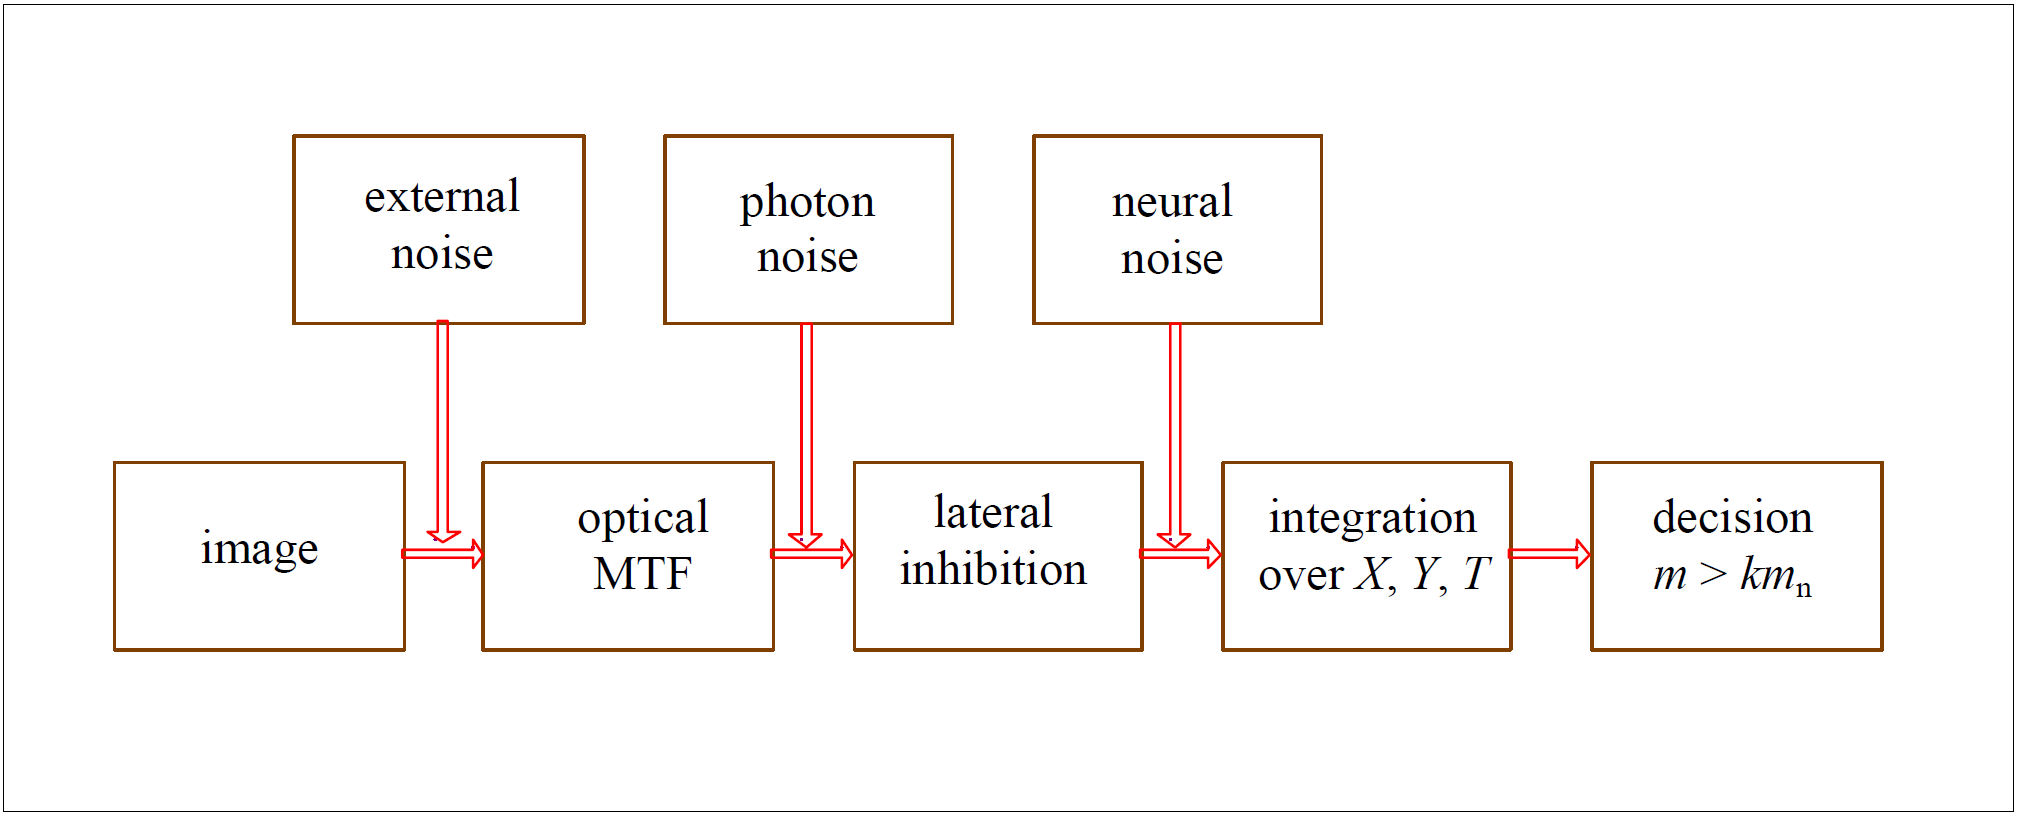
\includegraphics[width=0.48\textwidth]{CSF-Diagram.png}
    \caption{Block Diagram of the Contrast Sensitivity Model}
    \label{fig:csf_diagram}
\end{figure}
Figure\ref{fig:csf_diagram} shows a comprehensive model of contrast sensitivity.  
As we can see in the figure, there are three types of noises are taken into account. External noise, photon noise, neural noise, also there are two more function modules in the process pipeline. They are optical MTF (Optical modulation transfer function) and MTF (modulation transfer function) of lateral inhibition process. \\
Based on this module diagram, the equation \eqref{eq:mt_kmn} should be modified as
\begin{equation}
    \label{eq:modfied_mt_kmn}
    m_tM_{opt}(u)M_{lat}(u) = km_n
\end{equation}
Where $M_{opt}(u)$ is optical MTF, and $M_{lat}(u)$ is MTF of lateral inhibition process. Barten also derived the modulation of noise wave components $m_n$'s equation as below.
\begin{equation}
    \label{eq:m_n}
    m_n = 2\sqrt{\frac{\Phi_n}{XYT}}
\end{equation}
Where X,Y,T are spatial and temporal dimensions of the object. $\Phi_n$ is the special density of internal noise.\\
\begin{equation}
    \label{eq:XY}
    X = Y = (\frac{1}{X_o^2} + \frac{1}{X_{MAX}^2} + \frac{u^2}{N_{MAX}^2})^{-0.5}
\end{equation}
Where, $X_o$ is the angular size of object, $X_{MAX}$ is the maximum angular size of integration area of noise, $N_{MAX}$ is the maximum number of cycles over the eye can observe. \\
If we plug equation \eqref{eq:m_n} into equation \eqref{eq:modfied_mt_kmn}, we can obtains
\begin{equation}
    \label{eq:plugin1}
     m_tM_{opt}(u)M_{lat}(u) = 2k\sqrt{\frac{\Phi_n}{XYT}}
\end{equation}
The internal noise $\Phi_n$ is consisted with photon noise and neural noise.
\begin{equation}
    \label{eq:phi}
     \Phi_n = \Phi_{ph}M_{lat}^2(u) + \Phi_0
\end{equation}
then, plug equation \eqref{eq:phi} into equeation \eqref{eq:plugin1}, we get,
\begin{equation}
    \centering
    \label{eq:plugin2}
     m_tM_{opt}(u)M_{lat}(u) = 2k\sqrt{ \frac{\Phi_{ph}M_{lat}^2(u) + \Phi_0}{XYT}}
\end{equation}
then we can have,
\begin{equation}
    \centering
    \label{eq:mt2}
     m_t = \frac{2k}{M_{opt}(u)}\sqrt{ \frac{\Phi_{ph}M_{lat}^2(u) + \Phi_0}{XYTM_{lat}^2(u)}}
\end{equation}
From equation \eqref{eq:s_m}, we have,
\begin{equation}
    \centering
    \label{eq:s2}
     S(u) = \frac{1}{m_t(u)}  = \frac{M_{opt}(u)}{2k}\sqrt{ \frac{XYT}{\Phi_{ph} + \Phi_0/M_{lat}^2(u)}}
\end{equation}
At here, when we consider a binocular vision system, it is a two eyes observation, therefore, the internal noise factor should be corrected as $\sqrt{2}$, then equation \eqref{eq:m_n} should be modified to be,
\begin{equation}
    \label{eq:m_n_modified}
    m_n = \sqrt{2}\sqrt{\frac{\Phi_n}{XYT}}
\end{equation}
then equation \eqref{eq:s2} should be,
\begin{equation}
    \centering
    \label{eq:s3}
     S(u) = \frac{M_{opt}(u)}{\sqrt{2}k}\sqrt{ \frac{XYT}{\Phi_{ph} + \Phi_0/M_{lat}^2(u)}}
\end{equation}
If we plug equation \eqref{eq:XY} into equation \eqref{eq:s3}, we can get,
\begin{equation}
    \centering
    \label{eq:s4}
     S(u) = \frac{M_{opt}(u)/k}{\sqrt{\frac{2}{T}(\frac{1}{X_o^2}+\frac{1}{X_{MAX}^2}+\frac{u^2}{N_{MAX}^2})(\Phi_{ph}+\Phi_0/M_{lat}^2(u))}}
\end{equation}
Barten also provided the equations for optical MTF, photon noise, neural noise and MTF of lateral inhibition. They are shown as below.
\begin{equation}
    \centering
    \label{eq:m_opt}
    M_{opt} = e^{-2\pi^2\sigma^2u^2}
\end{equation}
where,
\begin{equation}
    \centering
    \label{eq:sigma}
    \sigma = \sqrt{\sigma_0^2+(C_{ab}d)^2}
\end{equation}
\begin{equation}
    \centering
    \label{eq:d}
    d = 5 -3 tanh(0.4logL)
\end{equation}

\begin{equation}
    \centering
    \label{eq:Phi_ph}
    \Phi_{ph} = \frac{1}{\eta pE}
\end{equation}
where $\eta$ is the quantum efficiency of eye, $E$ is the retinal illuminance in Troland, p is the photon conversion factor.
\begin{equation}
    \centering
    \label{eq:M_lat}
    M_{lat}(u) = \sqrt{1 - e^{-(u/u_0)^2}}
\end{equation}
Finally we have physical model of contrast sensitivity function: 
\begin{equation}
    \centering
    \label{eq:s4}
     S(u) = \frac{e^{-2\pi^2u^2(\sigma_0^2+(C_{ab}(5-3tanh(0.4logL)))^2)}/k}{\sqrt{\frac{2}{T}(\frac{1}{X_o^2}+\frac{1}{X_{MAX}^2}+\frac{u^2}{N_{MAX}^2})(\frac{1}{\eta pE}+\frac{\Phi_0}{1 - e^{-(u/u_0)^2}})}}
\end{equation}
Where the typical values used in this model are:\\
$\sigma_0 = 0.5$ arc min,  $C_{ab}=0.08$ arc min/mm, \\
$\eta = 0.03$, $p \approx 1.2\times10^6$, $k = 3.0$,\\
$X_{MAX} = 12\deg$, $N_{MAX}=15$cycles, $T = 0.1$sec,\\
$\Phi_0=3\times1^{-8}$ sec deg^2, $E \approx 14.7L^0.83$, $u_0=7$ cycles/deg.\\
$u$ is spatial frequency in $cycles/deg$, L is average luminance in $cd/{m^2}$. \\
After take above constant values into equation \eqref{eq:s4},we have a general formula which is more accurate.
\begin{equation}
    \centering
    \label{eq:s5}
     S(u) = \frac{5200e^{-0.0016u^2(1+100/L)^{0.08}}}{\sqrt{(1+\frac{144}{X_o^2}+0.64u^2)(\frac{63}{L^{0.83}}+\frac{1}{1-e^{-0.02u^2}})}}
\end{equation}

\subsection{Mathematical Approximation Formula Of Contrast Sensitivity Function}
Barten also published another formula in 1990 which has been widely used by other researchers.
It is shown as following equation.\\
\begin{equation}
    \centering
    \label{eq:barten1990}
     S(u) = aue^{-bu}\sqrt{1+ce^{bu}}
\end{equation}
Where $S$ is the contrast sensitivity, $u$ is spatial frequency in cycles per degree, a,b, and c are given by
\begin{equation}
    \centering
    \label{eq:a}
     a = \frac{540(1+0.7/L)^{-0.2}}{1+\frac{12}{X_o(1+u/3)}}
\end{equation}
\begin{equation}
    \centering
    \label{eq:b}
     b = 0.3(1+100/L)^{0.15}
\end{equation}
\begin{equation}
    \centering
    \label{eq:c}
     c = 0.06
\end{equation}


\subsection{Different Varieties of Contrast Sensitivity Functions}
Barten's research provided us fundamental basis of contrast sensitivity function. There are also some  simpler or enhanced varieties of contrast sensitivity functions have been developed as filer used in image processing and quality assessment. Here we introduce few of them which are widely used in modern engineering application and researching.

\subsubsection{Movshon's Model}
\begin{equation}
    \centering
    \label{eq:mannos}
     S(u) = au^be^{-cu}
\end{equation}
Where a = 75, b =0.2, and c = 0.8. This is simplest contrast sensitivity model.first described by Movshon and Kiorpes.

\subsubsection{Mannos-Skarison's Model}
\begin{equation}
    \centering
    \label{eq:mannos}
     S(u) = 2.6(0.0192+0.144u)e^{-(0.144u)^1.1}
\end{equation}
This equation developed by Mannos and Sakrison in 1974. It's widely used in application as it is easy to use.

\subsubsection{Daly's Model}
\begin{equation}
    \centering
    \label{eq:daly}
     S(u) = (\frac{0.008}{u^3}+1)^{-0.2}1.42ue^{-0.3u\sqtr{1+0.06e^{0.3u}}}
\end{equation}

\subsubsection{Ahumada's Model}
\begin{equation}
    \centering
    \label{eq:ahumada}
     S(u) = a_ce^{-(u/u_c)^2}-a_se^{-(u/u_s)^2}
\end{equation}
Where $a_c$ is the center, and $a_s$ is surround amplitude parameters. $u_c$ is the center, and $u_s$ is surround frequency cutoff parameters..  

\subsubsection{DoG's Model}
\begin{equation}
    \centering
    \label{eq:DoG}
     S(u) = e^{-(u/u_0)^2}-ae^{-(u/u_1)^2}
\end{equation}
This is called Difference of Gaussian function. It has good description of the sensitivity of individual retinal cell receptive field. 
\section{How to use Contrast sensitivity Function in An Image Processing Application}
So far we discussed the concepts contrast sensitivity function, the physical model of it and varieties of contrast sensitivity models. In this section we would like to discuss how can we apply contrast sensitivity function or filter in an application.

\subsection{Transformation of Coordinate System}
In general, if we have a source image $I(x,y)$, where (x,y) is pixel location, then after fourier transform we get spatial frequency domain image $\Theta(u,v)$, where, $u,v$ are spatial frequency on x, and y axis. However, CSF is in polar coordinate $r$, therefore, before apply CSF, we need to transform coordinate from x,y axis to polar coordinate by using following formula.
\begin{equation}
    \centering
    \label{eq:coor}
     r = \sqrt{u^2+v^2}
\end{equation}

\subsection{General process of applying Contrast sensitivity function in Application}
Let's say we have want create a color image difference metric for a pair of images, we can have below steps build in to the workflow to generate the metric.\\

\textbullet Transform image pairs into device independent
coordinates such as CIE XYZ .\\
    \textbullet Transform to opponent-color channels,luminance, red-green, yellow-blue.\\
    \textbullet Apply Fourier transform of opponent channels to get frequency domain data.\\
    \textbullet Filter frequency domain data by multiplying with Contrast Sensitivity Fiter\\
    \textbullet Apply Inverse Fourier transform to opponent space,and then into CIE XYZ coordinates.\\
    \textbullet Compute CIELAB value for each pixel.\\
    \textbullet Compute a pixel-to-pixel CIEDE2000 color difference error image.\\
    \textbullet Use image statistics such as mean, std. dev, median to get statistical error measurement.

\subsection{Example of use of Contrast Sensitivity Function in a NASA developed Algorithm}
The Spatial Standard Observer (SSO) software algorithm was developed by NASA that incorporates a simple model of human visual sensitivity to spatial contrast. The algorithm was specifically created for display applications and the identification of display MURA. This algorithm has been adapted for use in some image analysis software to identify and grade arbitrary display data
captured by an imaging photometer or colorimeter. Main features those are included in this model are: spatial frequency, which represent how fast spatial contrast varies, orientation ,which show the angular orientation of the spatial contrast relative to the viewing plane defined by human eyes, and the observer’s distance from the display being viewed. \\
Generally, the analysis technology can be applied to either a photopic or colorimetric measurement image; because the analysis method generates useful data for both brightness and color.\\
A summary of SSO algorithm is described below.\\
• The input to the algorithm is a pair of images: the test image and a reference image.\\
• The test image is the initial imaging colorimeter measurement, containing potential
mura defects.\\
• The reference image is computed from the test image using a low-pass filter
designed to eliminate the mura.\\
• The difference between test and reference images is filtered by a contrast sensitivity
function (CSF).\\
• The filtered image is then multiplied by an aperture function.\\
• The aperture function models the decline in human visual sensitivity with
distance from the point of fixation.\\
• The final step is a non-linear pooling of the resulting image over space to produce the
JND image.\\

As we can see the contrast sensitivity function plays a key role within SSO algorithm to perform the a measurement of the visibility of different spatial frequencies at different orientations. It models the decline in human visual sensitivity at higher spatial frequencies and at very low frequencies, as well as the lower sensitivity at oblique orientations.
Display defect detection performed using this type of system that analysis an effective means of obtaining additional information about display image quality that extends to other analysis techniques. This analysis system can be applied
to any display type, including LCD, LED, and OLED displays.

\section{Discussion}
Contrast sensitivity function is measure of fundamental spaiochromatic properties of human visual system. it can play a key role not just in image quality assessment, but also could be used in display quality control and performance measurement. In an display quality assessment system, display luminance non-uniformity is common issue which directly impact display product yield. It has been an issue to relay on subjective human observation to check display luminance uniformity based on human vision. It takes long time and different inspectors could give different evaluation results. An accurate and speedy objective assessment system is needed. In this kind of system a contrast sensitivity function is a needed to improve the assessment result accuracy, and remove the varieties of human vision effect.

\section{Future Work}


\end{document}
